\chapter[Registro de Requisitos na Ferramenta RallyDev]{Registro de Requisitos na Ferramenta RallyDev}
\label{chap:ferramenta}
	Todos os requisitos elicitados foram registrados e monitorados na ferramenta RallyDev, pela organização proposta no \emph{Scaled Agile Framework}. A seguir, é possível contemplar imagens da utilização da ferramenta no contexto do projeto.
	\begin{figure}[H]
		\centering
		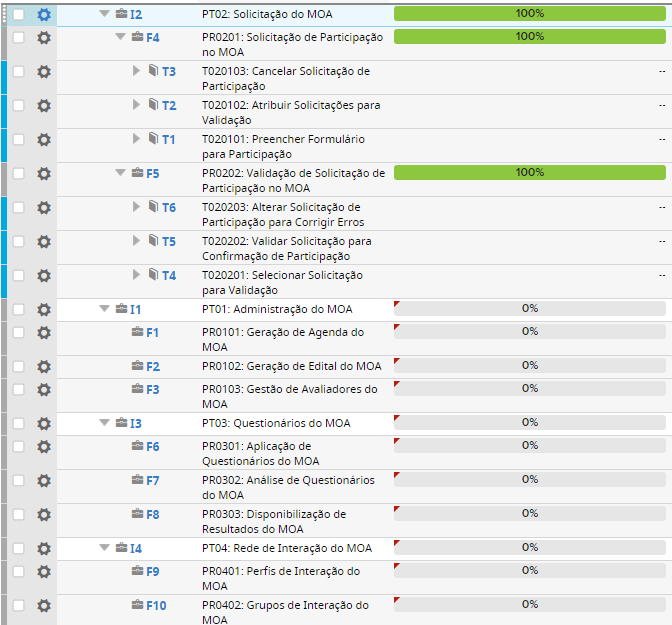
\includegraphics[scale=0.85]{rally_rastreabilidade_01}
		\caption[Requisitos Registrados na Ferramenta RallyDev (Rastreável)]{Requisitos Registrados na Ferramenta RallyDev (Rastreável).}
		\label{fig:rastreabilidadeum}
	\end{figure}
	\begin{landscape}
		\vspace*{\fill}
		\begin{figure}[H]
			\centering
			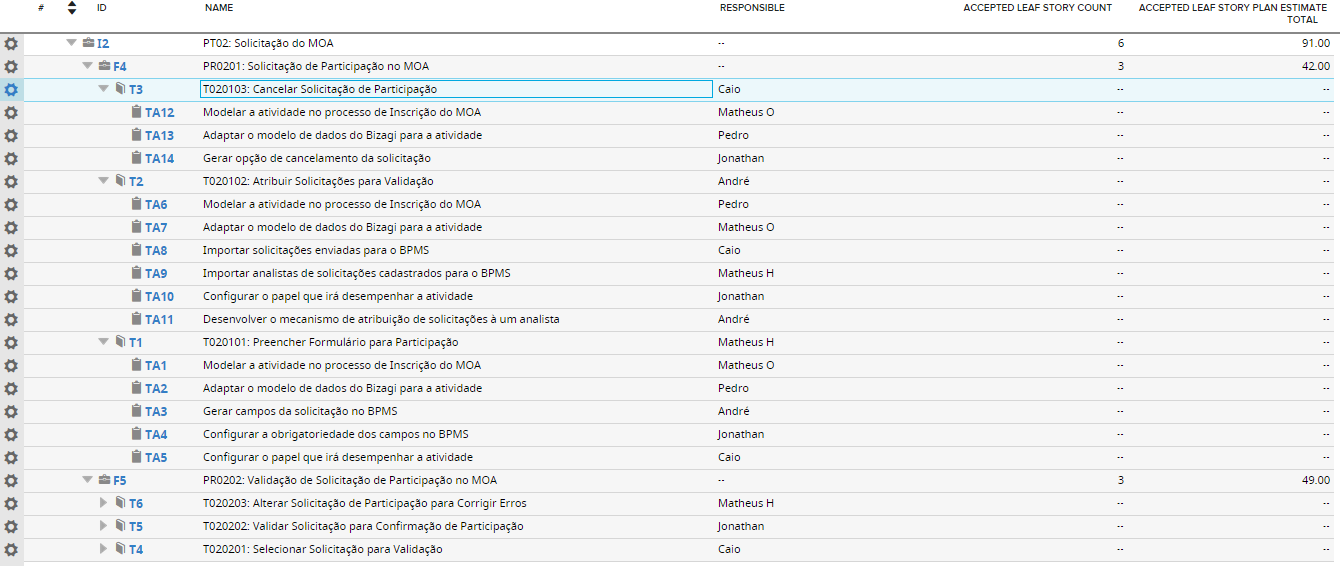
\includegraphics[scale=0.65]{rally_rastreabilidade_02}
			\caption[Requisitos associados à Tarefas na Ferramenta RallyDev (Rastreável)]{Requisitos associados à Tarefas na Ferramenta RallyDev (Rastreável).}
			\label{fig:rastreabilidadedois}
		\end{figure}
		\vspace*{\fill}
	\end{landscape}
	\begin{landscape}
		\vspace*{\fill}
		\begin{figure}[H]
			\centering
			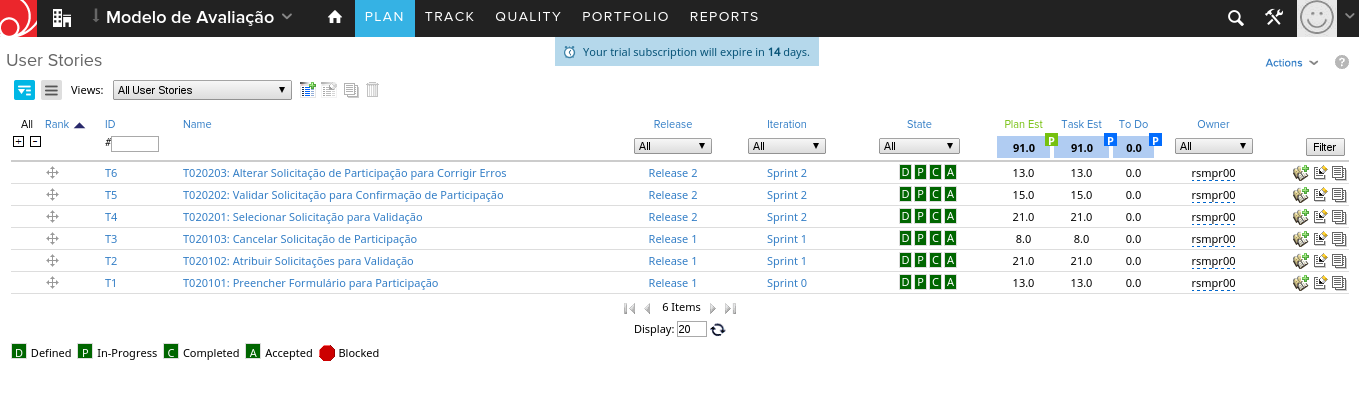
\includegraphics[scale=0.50]{rally_us}
			\caption[Backlog de Time (Histórias de Usuário) na Ferramenta RallyDev]{Backlog de Time (Histórias de Usuário) na Ferramenta RallyDev.}
			\label{fig:rallyus}
		\end{figure}
		\vspace*{\fill}
	\end{landscape}